 % This file is public domain.

\documentclass[a4paper]{report}

\usepackage[landscape,margin=15pt]{geometry}
\usepackage{color}
\usepackage{flowfram}
\usepackage[colorlinks]{hyperref}

\renewcommand{\familydefault}{cmss}

\adjustheight{\textheight}

\onecolumninarea[1,2]{0.5\textwidth}{\textheight}{0.5\textwidth}{0pt}
\twocolumninarea[>2]{0.5\textwidth}{\textheight}{0.4\textwidth}{0pt}


\newdynamicframe{0.4\textwidth}{\textheight}{0pt}{0pt}[left]

\dfchaphead*{left}
\renewcommand{\DFchapterstyle}[1]{%
\raggedright\Huge\slshape\MakeUppercase{#1}\par}

%\vtwotone[1]{0.6\paperwidth}{[cmyk]{0.65,0.13,0,0}}{backleft}%
%{0.4\paperwidth}{[cmyk]{0.94,0.54,0,0}}{backright}
%
%\vtwotonetop{1cm}{0.6\paperwidth}{[cmyk]{0.65,0.13,0,0}}{topleft}%
%{0.4\paperwidth}{[cmyk]{0.94,0.54,0,0}}{topright}

\newstaticframe{0.4\textwidth}{39cm}{2pt}{0pt}[head]

\newstaticframe{0.4\textwidth}{34cm}{2pt}{0pt}[title]

\newstaticframe{\textwidth}{0.8\textheight}{0pt}{0pt}[img]

\newstaticframe{\textwidth}{0.2\textheight}{0pt}{-\footskip}[logo]

\pagestyle{empty}

\renewcommand{\chapterfirstpagestyle}{empty}

\newstaticframe{\textwidth}{\headheight}{0pt}{-\footskip}[footer]

\setstaticcontents*{footer}{%
University of Luxembourg}

\newcommand{\env}[1]{\texttt{#1}}
\newcommand{\cmdname}[1]{\texttt{\symbol{92}#1}}
\newcommand{\meta}[1]{\textnormal{\textless\textit{#1}\textgreater}}

\usepackage{graphicx}

\begin{document}

\setstaticcontents*{head}{\small\slshape\MakeUppercase{ESTEC Contract Number 4000128969/19/NL/AS}}

\setstaticcontents*{title}{\Huge\slshape\MakeUppercase{FAQAS:\\ Verifying and improving\\ test suites}}

\setstaticcontents*{img}{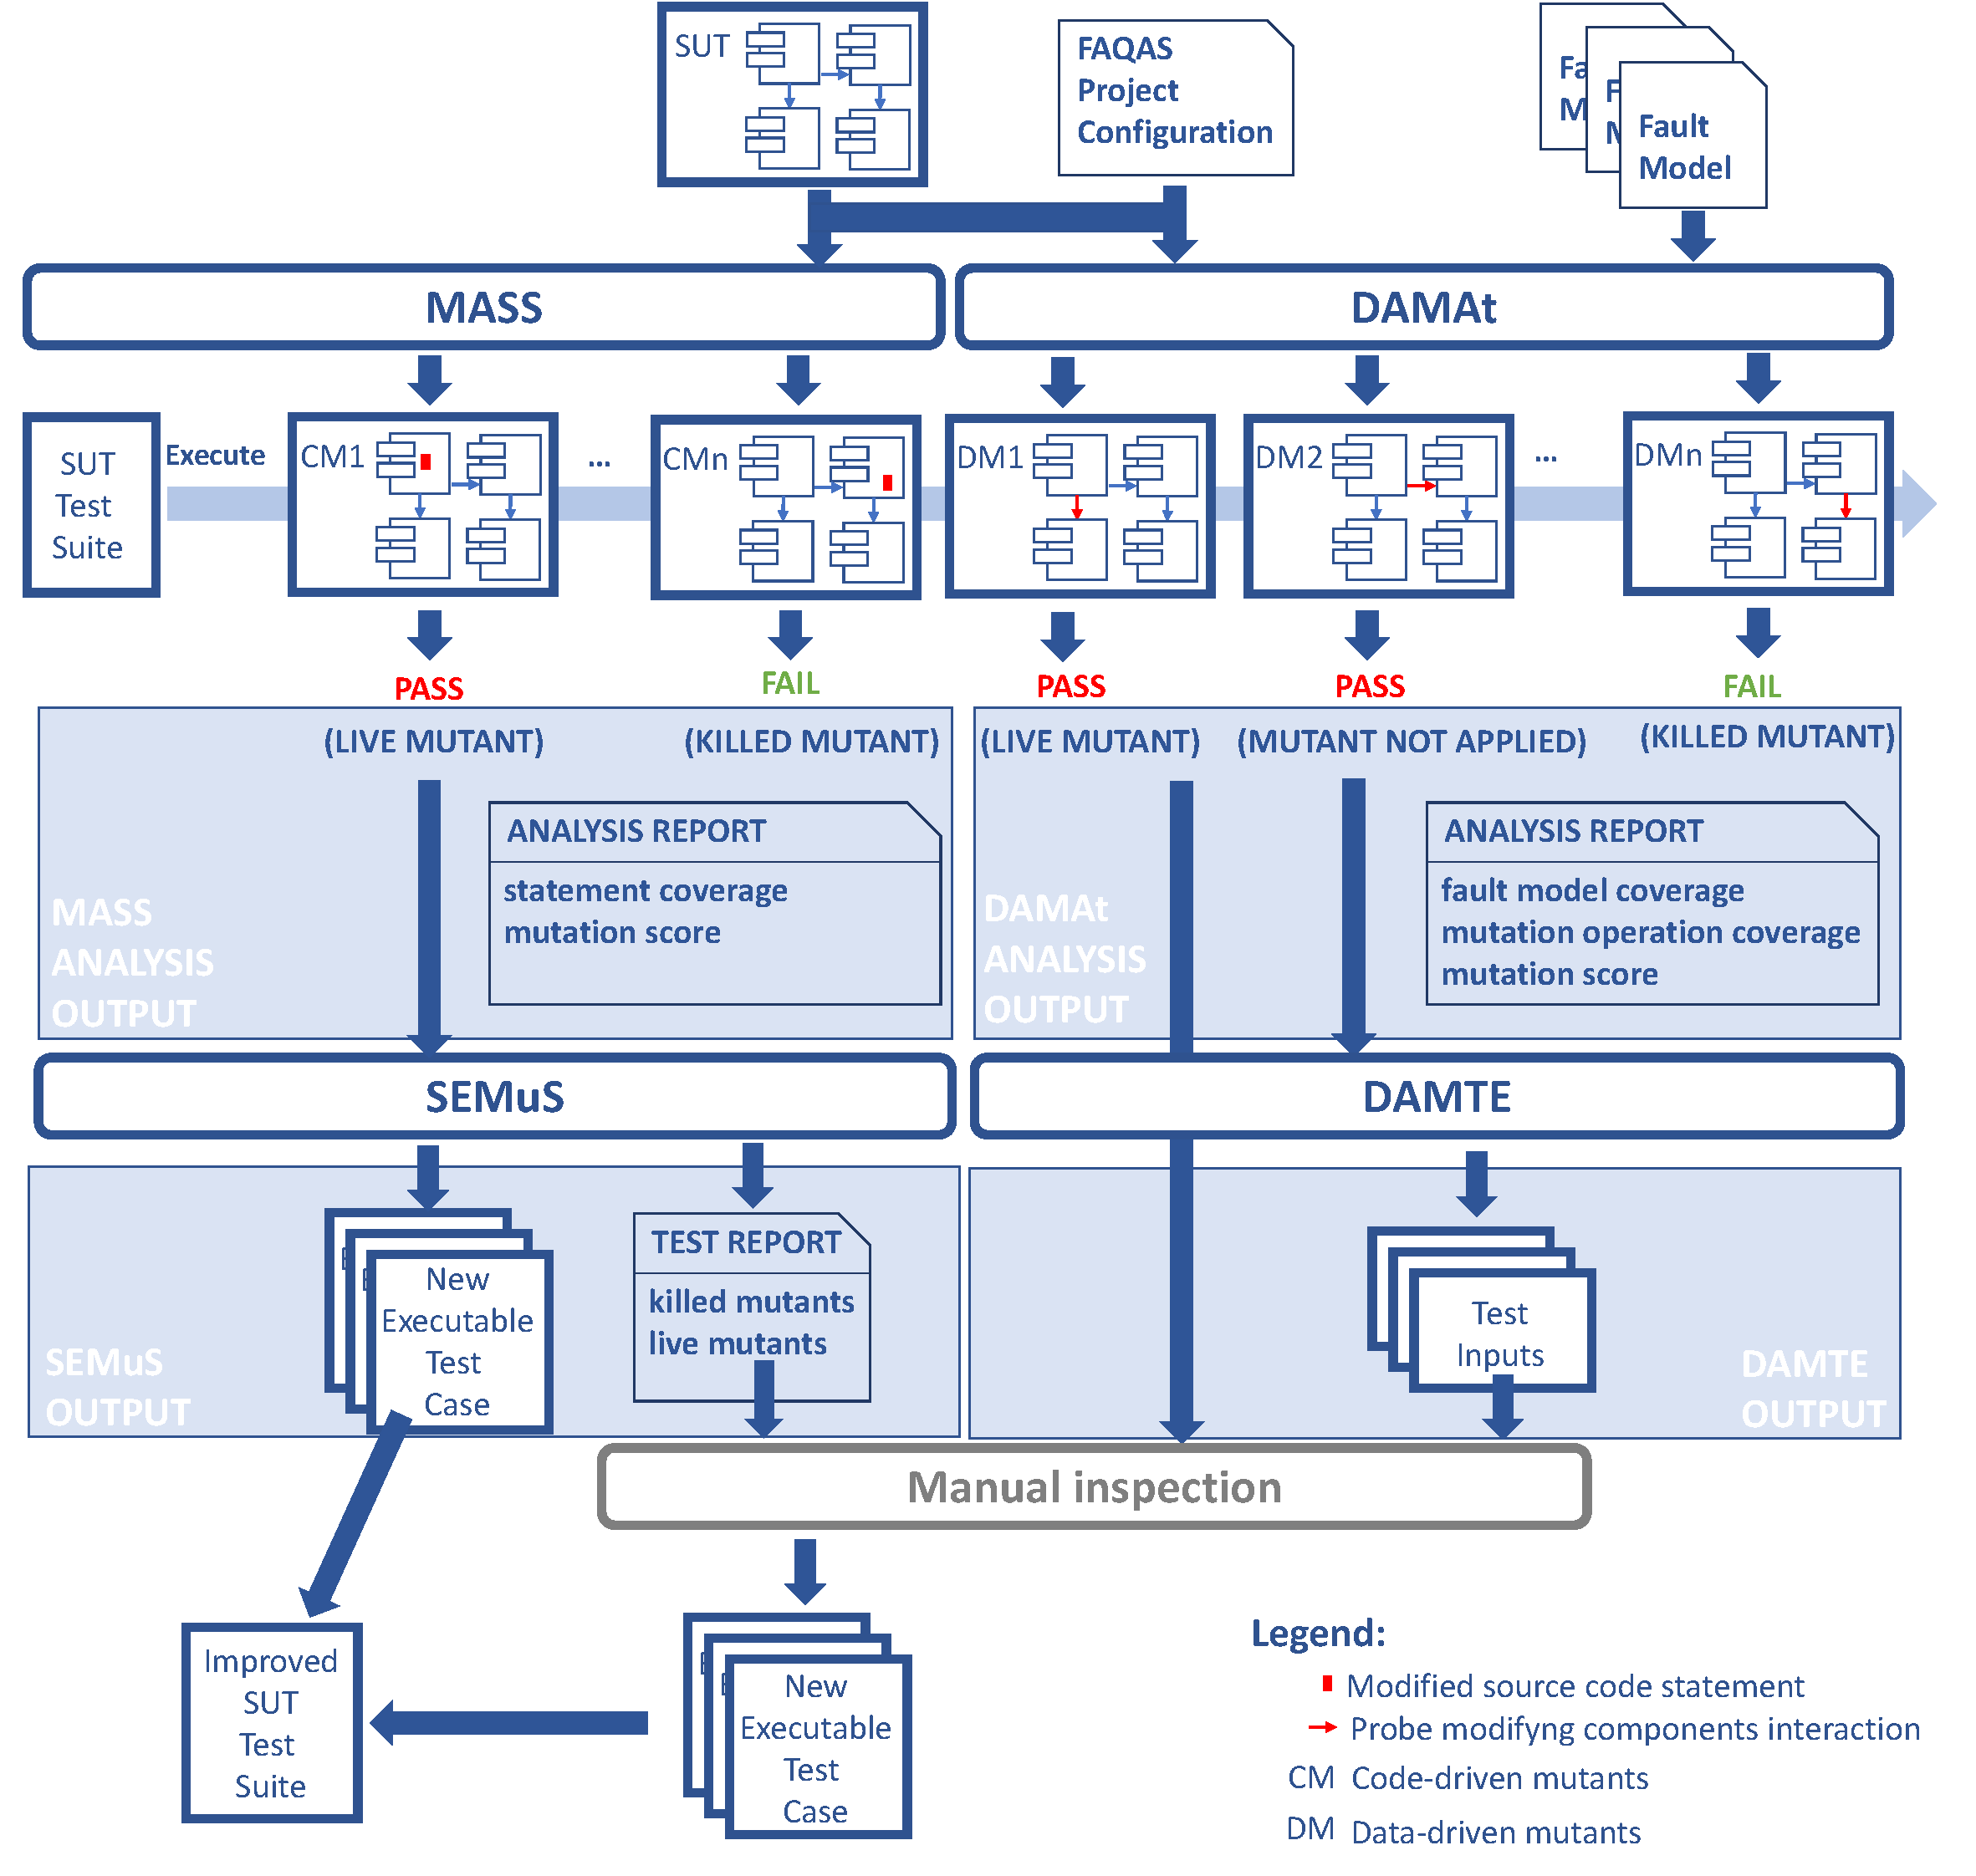
\includegraphics[width=14cm]{FAQAS-overview.pdf}}

\setstaticcontents*{logo}{University of Luxembourg. SnT Centre. Contact: Technology Transfer Office, snt-tto@uni.lu. \hspace{10.5cm} 
\includegraphics[width=1.5cm]{logo-uni-lu.pdf}\hspace{1.5mm}
\includegraphics[width=2cm]{logo-snt.pdf} }

%{\noindent
%\slshape\Huge\MakeUppercase{A Sample Brochure}\par
%\vskip0.5in
%\noindent\large\MakeUppercase{Nicola Talbot}\\
%}

%\chapter{}

From spacecrafts to ground stations, software has a prominent role in space systems; for this reason, the success of space missions depends on the quality of the system hardware as much on the dependability of its software --- but, \textbf{how to systematically verify the quality of large test suites?} 

To address the question above, the FAQAS project consortium built an efficient toolset to 
\textbf{measure} how a test suite detects faults automatically injected into the software system under test (SUT). Also, the FAQAS toolset automatically \textbf{generates new test cases} that discover faults missed by the original SUT test suite. The targeted SUT includes flight software and ground processing software.
The FAQAS toolset can be used by software or ISVV suppliers to enhance their validation  \&  verification methodologies.
The FAQAS consortium includes the \textbf{\emph{SnT Centre of the University of Luxembourg}}\footnote{https://wwwen.uni.lu/snt}, \textbf{\emph{Gomspace Luxembourg}}\footnote{https://gomspace.com/} (GSL) and \textbf{\emph{OHB Luxspace}}\footnote{https://luxspace.lu/} (LXS).

The FAQAS toolset includes 
\textbf{\emph{MASS}} (Mutation Analysis for Space Software, TRL 5), 
\textbf{\emph{DAMAt}} (DAta-driven Mutation Analysis with Tables, TRL 4), 
\textbf{\emph{SEMuS}} (Symbolic Execu\-tion-based MUtant analysis for Space software, TRL 3),
and \textbf{\emph{DAMTE}} (DAta-driven Mutation TEsting, TRL 2).
It generates modified versions of the SUT, some derived by modifying the implementation of the software (code-driven mutants) others by integrating an API that alters the messages exchanged by the SUT components (data-driven mutants). 
Test suite effectiveness is measured as the percentage of mutants discovered by the test suite (i.e., the \textbf{mutation score}). The mutants that are not discovered by the test suite (i.e., it does not fail) are said to be \emph{live} and point out shortcomings.

\textbf{\emph{MASS}} generates code-driven mutants. It integrates a pipeline of solutions that make mutation analysis feasible with large SUTs. MASS (1) automatically identifies trivially equivalent mutants using an ensemble of compiler optimization options, (2) estimates the mutation score through sampling with a fixed size confidence interval approach, (3) identifies equivalent mutants based on code coverage. 
MASS reports the set of live mutants, killed mutants (i.e., discovered by the test suite), statement coverage, and the mutation score.

\textbf{\emph{DAMAt}} generates data-driven mutants. 
It relies on fault models that specify how to mutate the data exchanged by SUT components through data-driven mutation operators. 
DAMAt enables the simulation of faults that affect simulated components (e.g., sensors), which is not feasible with code-driven mutation analysis. 
DAMAt reports the following test suites' pitfalls: message types never tested,
mutants not applied (i.e., mutants that could not alter any data because the data they target was \textbf{erronously} never exercised by the SUT),
live mutants (i.e., mutants that successfully alter the data but are not detected by the test suite because it lacks appropriate assertions or does not cover the required inputs).
% killed mutants (i.e., successfully alter the data, and lead to test case failures), the set of 
%also, it provides information useful to draft a verification report, which includes the fault model coverage (i.e., percentage of fault models with at least one mutant applied), the mutation operation coverage (i.e., percentage of mutants applied), and the mutation score.

\textbf{\emph{SEMuS}} automatically generates executable unit test cases based on code-driven mutation analysis results. The generated unit test cases kill mutants not detected by the original test suite. The generated test cases include test oracles that enable the detection of faults affecting the SUT.

%SEMuS takes as input the list of live mutants detected by MASS. It generates a set of additional test cases that can be integrated into the SUT test suite. Also, it reports the list of killed mutants and the list of mutants that remain live (i.e., for which SEMuS did not generate a test case that kill them). Live mutants shall be manually inspected by engineers to either determine if they are equivalent or to manually derive a test case capable of killing them.

\textbf{\emph{DAMTE}} is a manual procedure supported by an automated symbolic execution toolset; it automatically identifies the test inputs that make SUT components exchange the data targeted by data-driven mutation operators. The derived test inputs can then be manually integrated into the SUT test suite.
 
The activity also included an extensive empirical evaluation demonstrating the feasibility, effectiveness, and scalability of the proposed toolsets in the space context. The toolset has been \textbf{\emph{positively evaluated}} by industry partners; indeed, it enabled the discovery of defects and proved to improve the quality of the development process.

%\chapter{Setting up Frames}
%
%This is column~\thedisplayedframe.
%
%The \textsl{flowfram} package provides three types of frame:
%{flow frames}, {static
%frames} and {dynamic frames}.
%
%\section*{Flow Frames}
%
%\labelflow{flow:flowframe}
%The flow frame is the principle type of frame.
%The text of the \env{document} environment will flow from
%one frame to the next in order of definition. Each
%flow frame has an associated width, height,
%position on the page, and optionally a border.
%
%It is recommended that all the flow frames in a document
%have the same width, otherwise problems may occur
%when a paragraph spans to flow frames of unequal
%widths. This is because \TeX's output routine does not
%register the change in \cmdname{hsize} until it reaches
%a paragraph break. If it is absolutely necessary for
%flow frames to have unequal widths, judicious use of
%\cmdname{framebreak} is required.
%
%\section*{Static Frames}
%
%A static frame is a rectangular area in which text neither
%flows into, nor flows out of.  The contents must be set
%explicitly, and once set, the contents of the static frame will
%remain the same on each page until it is explicitly
%changed.  Thus, a static frame can be used, for example, to make
%a company logo appear in the same place on every page.
%
%\section*{Dynamic Frames}
%
%A dynamic frame is similar to a static frame, but its contents
%are re-typeset on each page. (A static frame stores its
%contents in a savebox, whereas a dynamic frame stores its
%contents in a macro).
%
%This is column~\thedisplayedframe.
%
%\chapter{Frame Attributes}
%\label{sec:modattr}
%
%Once you have defined the {flow frames}, {static frames} and
%{dynamic frames}, their attributes can be changed.
%The three types of frame mostly have the
%same set of attributes, but some are specific to a certain type.
%The available attributes are as follows
%(\textsuperscript{\textbf{F}} indicates the key is
%only available for {flow frames},
%\textsuperscript{\textbf{S}} indicates the key is only available
%for {static frames}
%and \textsuperscript{\textbf{D}} indicates the key
%is only available for {dynamic frames}):
%
%\begin{description}
%\item[width=\meta{length}]\mbox{}\par  The width of the frame.
%
%\item[height=\meta{length}]\mbox{}\par The height of the frame.
%
%\item[x=\meta{length}]\mbox{}\par The x-coordinate of the frame.
%
%\item[y=\meta{length}]\mbox{}\par The y-coordinate of the frame.
%
%\item[border=\meta{style}]\mbox{}\par The style of the border around the
%frame, this can take the values: \texttt{none} (no border),
%\texttt{plain} (plain border) or the name of a \LaTeX\
%frame making command without the preceding backslash.
%The value \texttt{fbox} is equivalent to \texttt{plain}.
%
%\item[offset=\meta{offset}]\mbox{}\par The border offset, if it is a
%user-defined border.  This is the distance from the outer
%edge of the left hand border to the left edge of the
%bounding box of the text inside the border.  The \textsl{flowfram}
%package is able to compute the border for
%known frame making commands.
%If you define your own frame making command, you may need to
%specify the offset explicitly, or the frames
%may end up shifted to the right or left.
%
%\item[bordercolor=\meta{colour}]\mbox{}\par The colour of the border
%if you are using a standard frame making command.
%The colour can either be specified as, e.g.\ \texttt{green},
%or including the colour model, for example
%\verb/[rgb]{0,1,0}/.
%
%\item[textcolor=\meta{colour}]\mbox{}\par The text colour for that
%frame. Again, the colour can either be specified as,
%e.g.\ \texttt{green}, or including the colour model,
%for example \verb/[rgb]{0,1,0}/.
%
%\item[pages=\meta{page list}]\mbox{}\par The {list of
%pages} for which the frame
%should appear. This can either have the values: \texttt{all},
%\texttt{even}, \texttt{odd} or \texttt{none} (the latter
%removes the frame from that point on---useful if you
%have multiple pages with the same number), or it can be a
%comma-separated list of single pages, or
%{page ranges}.
%
%\item[margin=\meta{side}\textsuperscript{F}]\mbox{}\par The side of
%the flow frame that its corresponding margin should go on. This
%can take the values \texttt{left} or \texttt{right}.
%
%\item[clear=\meta{boolean}\textsuperscript{S}] If this value
%is set, the static frame will be cleared at the start of the
%next page.
%
%\item[style=\meta{cmd}\textsuperscript{D}]\mbox{}\par This should be
%the name of a command \emph{without} the preceding backslash,
%to be applied to the contents of the specified dynamic frame.
%The command may either be a declaration, for example \verb/style=large/
%which will set the contents of all the dynamic frames in a
%large font, or it can be a command that takes a single argument,
%for example \verb/style=textbf/
%which will make the text for all the dynamic frames come out in
%bold.  To unset a style, do \verb/style=none/.
%
%\end{description}
%
%\chapter{Miscellaneous}
%
%\section*{Page Layout}
%
%The \textsl{flowfram} package has the package option \texttt{draft}
%which will draw the {bounding boxes} for
%each frame defined.  At the bottom right of each
%bounding box (except for the bounding box denoting the
%typeblock), a marker will be shown to indictate the type
%of frame, its IDN and its IDL.
%
%You can see the layout for the current page (irrespective of
%whether or not the \texttt{draft} option has been set) using
%the command:\newline
%\cmdname{flowframeshowlayout}
%
%The headers and footers will appear as usual (but will not
%be shown in draft mode), according to the format given by
%\cmdname{pagestyle}.
%
%\section*{Frame Stacking Order}
%
%\labelflow{flow:stacking}
%The material on each page is placed in the following order:
%\begin{enumerate}
%\item Each static frame defined for that page in ascending
%order of IDN.
%
%\item Each flow frame defined for that page in ascending
%order of IDN.
%
%\item Each dynamic frame defined for that page in ascending
%order of IDN.
%
%\item {Bounding boxes} if the \texttt{draft}
%package option has been used.
%\end{enumerate}
%
%This ordering can be used to determine if you want something
%to overlay or underlay everything else on the page.
%
%\section*{Prematurely Ending a Flow Frame}
%
%You can force text to move immediately to the next defined
%flow frame using one of the standard \LaTeX\ page breaking commands
%which  work in an analogous way to the way they
%work in standard two column mode.
%
%The command \cmdname{framebreak} is provided for situations
%where a paragraph spans two flow frames
%of different widths, as \TeX's output routine does not
%adjust to the new value of \cmdname{hsize} until the last
%paragraph of the previous frame has ended. As a
%result, the end of the paragraph at the beginning of the new
%flow frame retains the width of the previous flow frame.
%
%If you want to start a new page, rather than simply move to the
%next frame, use the command\newline
%\cmdname{finishthispage}.
%
%\section*{Floats}
%
%\labelflow{flow:floats}
%Since floats (such as figures and tables) can only go in
%{flow frames}, this package provides
%the additional environments:
%\env{staticfigure} and
%\env{statictable} which can be used in static frames
%and dynamic frames. Unlike their \env{figure} and
%\env{table} counterparts, they are fixed in place, and
%so do not take an optional placement specifier. The
%\cmdname{caption} and \cmdname{label} commands can
%be used within \env{staticfigure} and \env{statictable} as
%usual.
%
%The standard \env{figure} and \env{table} commands will
%behave as usual in the flow frames, but their starred versions,
%\env{figure*} and \env{table*} behave no differently
%from \env{figure} and \env{table}.
%
%\section*{Global Values}
%
%The following macros can be changed using\linebreak \cmdname{renewcommand}:
%
%\begin{itemize}
%\item \cmdname{setffdraftcolor}
%
%This sets the colour of the bounding box
%when it is displayed in draft mode.
%
%\item
%\cmdname{setffdrafttypeblockcolor}
%
%This sets the colour of
%the bounding box of the typeblock when it is displayed
%in draft mode.
%
%\item \cmdname{fflabelfont}
%
%This sets the font size for the bounding box markers in
%draft mode.
%
%\end{itemize}
%
%The following are lengths, which can be changed using
%\cmdname{setlength}:
%
%\begin{itemize}
%\item \cmdname{fflabelsep}
%
%This is the distance from the right hand side of the
%bounding box at which to place the bounding box marker.
%
%\item \cmdname{flowframesep}
%
%This is the gap between the text of the frame and
%its border, for the standard border types.
%
%\item \cmdname{flowframerule}
%
%This is the width of the frame's border, if using
%a border given by a frame making command that uses \cmdname{fboxsep}
%to set its border width.
%
%\item \cmdname{columnsep}
%
%This is the horizontal distance between flow frames when using one of the
%\cmdname{Ncolumn} type of commands
%
%\item \cmdname{vcolumnsep}
%
%This is the vertical distance between the flow frames and the static or
%dynamic frame when using one of the \cmdname{Ncolumntop} type of commands.
%\end{itemize}
%
%\label{lastpage}
\end{document}
